\documentclass[twocolumn]{article}

\usepackage[style=nature, backend=biber]{biblatex}
\def\bibsection{\sectionTitle{References}}
\addbibresource{refs.bib}

\usepackage{filecontents}
\usepackage{array,booktabs,csvsimple,longtable,tabularx}
\usepackage{tabu}
\usepackage[utf8]{inputenc}
\usepackage{listings}
\usepackage{color} %red, green, blue, yellow, cyan, magenta, black, white
\definecolor{mygreen}{RGB}{0,0.6,0} % color values Red, Green, Blue
\definecolor{mygray}{RGB}{0.47,0.47,0.33}
\definecolor{myorange}{RGB}{0.8,0.4,0}
\definecolor{mywhite}{RGB}{0.98,0.98,0.98}
\definecolor{myblue}{RGB}{0.01,0.61,0.98}
\usepackage{graphicx}
\usepackage{etoolbox}
\usepackage[normalem]{ulem}    
\usepackage{tikz}
\usepackage{float}
\usepackage{subcaption}
\usetikzlibrary{shapes.geometric, intersections, patterns}
\usepackage{pgf, pgfcore, pgfplots, pgfplotstable}
\usepgfplotslibrary{fillbetween}
\pgfplotsset{compat=newest}
\usepackage{pgfplotstable, dcolumn}

\newcommand{\ra}[1]{\renewcommand{\arraystretch}{#1}}
\newcommand{\rpm}{\raisebox{.2ex}{$\scriptstyle\pm$}}

%% https://tex.stackexchange.com/questions/211415/how-to-set-up-listings-for-use-code-from-arduino
\newcommand*{\FormatDigit}[1]{\ttfamily\textcolor{mygreen}{#1}}
%% https://tex.stackexchange.com/questions/32174/listings-package-how-can-i-format-all-numbers
\lstdefinestyle{FormattedNumber}{%
	literate=*{0}{{\FormatDigit{0}}}{1}%
	{1}{{\FormatDigit{1}}}{1}%
	{2}{{\FormatDigit{2}}}{1}%
	{3}{{\FormatDigit{3}}}{1}%
	{4}{{\FormatDigit{4}}}{1}%
	{5}{{\FormatDigit{5}}}{1}%
	{6}{{\FormatDigit{6}}}{1}%
	{7}{{\FormatDigit{7}}}{1}%
	{8}{{\FormatDigit{8}}}{1}%
	{9}{{\FormatDigit{9}}}{1}%
	{.0}{{\FormatDigit{.0}}}{2}% Following is to ensure that only periods
	{.1}{{\FormatDigit{.1}}}{2}% followed by a digit are changed.
	{.2}{{\FormatDigit{.2}}}{2}%
	{.3}{{\FormatDigit{.3}}}{2}%
	{.4}{{\FormatDigit{.4}}}{2}%
	{.5}{{\FormatDigit{.5}}}{2}%
	{.6}{{\FormatDigit{.6}}}{2}%
	{.7}{{\FormatDigit{.7}}}{2}%
	{.8}{{\FormatDigit{.8}}}{2}%
	{.9}{{\FormatDigit{.9}}}{2}%
	%{,}{{\FormatDigit{,}}{1}% depends if you want the "," in color
	{\ }{{ }}{1}% handle the space
	,%
}


\lstset{%
	backgroundcolor=\color{mywhite},   
	basicstyle=\footnotesize,       
	breakatwhitespace=false,         
	breaklines=true,                 
	captionpos=b,                   
	commentstyle=\color{red},    
	deletekeywords={...},           
	escapeinside={\%*}{*)},          
	extendedchars=true,              
	frame=shadowbox,                    
	keepspaces=true,                 
	keywordstyle=\color{myorange},       
	language=Octave,                
	morekeywords={*,...},            
	numbers=left,                    
	numbersep=5pt,                   
	numberstyle=\tiny\color{mygray}, 
	rulecolor=\color{black},         
	rulesepcolor=\color{myblue},
	showspaces=false,                
	showstringspaces=false,          
	showtabs=false,                  
	stepnumber=2,                    
	stringstyle=\color{myorange},    
	tabsize=2,                       
	title=\lstname,
	emphstyle=\bfseries\color{blue},%  style for emph={} 
}    

%% language specific settings:
\lstdefinestyle{Arduino}{%
	style=FormattedNumber,
	keywords={void},%                 define keywords
	morecomment=[l]{//},%             treat // as comments
	morecomment=[s]{/*}{*/},%         define /* ... */ comments
	emph={HIGH, OUTPUT, LOW},%        keywords to emphasize
}

\newtoggle{InString}{}% Keep track of if we are within a string
\togglefalse{InString}% Assume not initally in string

\newcommand{\classname}{EE3: Introduction to Electrical Engineering}
\newcommand{\project}{- Path Following Robot -}
\newcommand{\authorname}{Brian Dionigi Raymond\\Kevin Ke-En Sun}
\newcommand{\instructor}{Prof. Briggs}

\newcommand{\sectionTitle}[1]{ {\large\textbf{\uline{#1}}} \\ \vspace{1.5em} }
\newcommand{\subsectionTitle}[1]{ {\hspace{2em}\uline{#1}} \\ \vspace{1em} }


\begin{document}
		
	\begin{center}
		{\LARGE \textsc{\classname \\ \project} \\ \vspace{4pt}}
		\rule[13pt]{0.5\textwidth}{1pt} \\ %\vspace{150pt}
		{\authorname \\ \vspace{2pt}
			Instructor: \instructor \\ \vspace{2pt}
			\today \\ \vspace{2pt}
		}
	\end{center}	
	
	\begin{flushleft}
		\sectionTitle{Introduction}
		
		\hspace{1em}The goal of the project was to design a car able to follow a path represented by a black line on a white piece of paper. A PID function will be used to control the steering of the car. In addition, the car must be able to sense the stop at the end of the track and automatically stop. The extra credit portion of this project was to be able to sense, using speed sensors, when the motors have come to a stop and signal to the car that it must momentarily drive the motors at a higher duty cycle to get them moving again. \\
		\hspace{1em} The car uses three sensors to detect where to go on the path, one on the front, one on the right, and one on the left. The sensors work by using an IR LED that reflects IR light off the ground and into a phototransistor. They are connected to each other as shown in Figure \ref{fig:circuitSensors}. A phototransistor works like a transistor; a transistor is like a switch. A transistor has three terminals: a base, an emitter, and a collector. When a voltage is applied to the base that is relatively higher than the voltage on the emitter, current is allowed to flow from the emitter to the collector. If the voltage applied to the base is relatively lower than the voltage on the emitter, then no current is allowed to flow. A phototransistor is different from a regular transistor, however, in that the base is sensitive to light as opposed to voltage. When light is shown on the base, current is allowed to flow. If no light is being shown then no current flows. An emitter follower setup was used for the sensors (signal response is low in absence of IR light and high in its presence). \\ \vspace{1em}
		
		\begin{figure}[H]

			\centering{\textbf{Circuits for Path Sensing and Movement}\par\medskip}
			{\begin{subfigure}[b]{0.45\textwidth}
				\frame{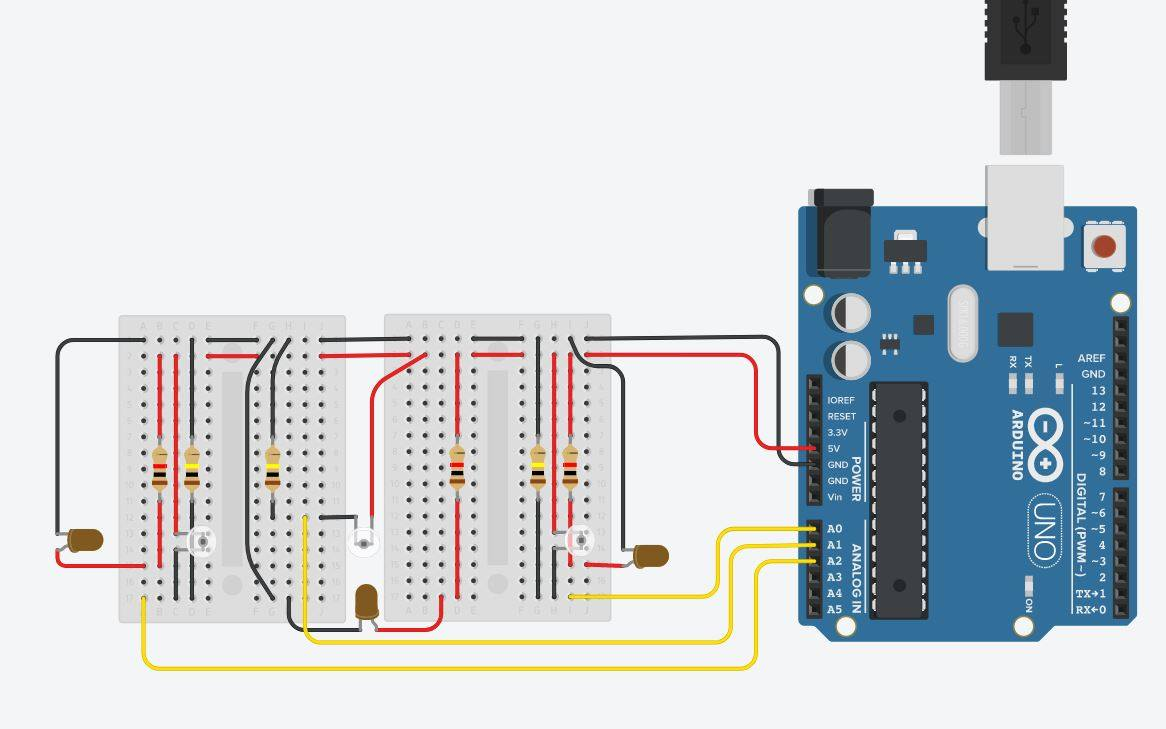
\includegraphics[width=1\columnwidth, keepaspectratio]{CircuitSensors.jpg}}
				\caption{IR LED and Phototransistor Circuit}
				\label{fig:circuitSensors}
			\end{subfigure}\\ \vspace{1em}%
			\begin{subfigure}[b]{0.45\textwidth}
				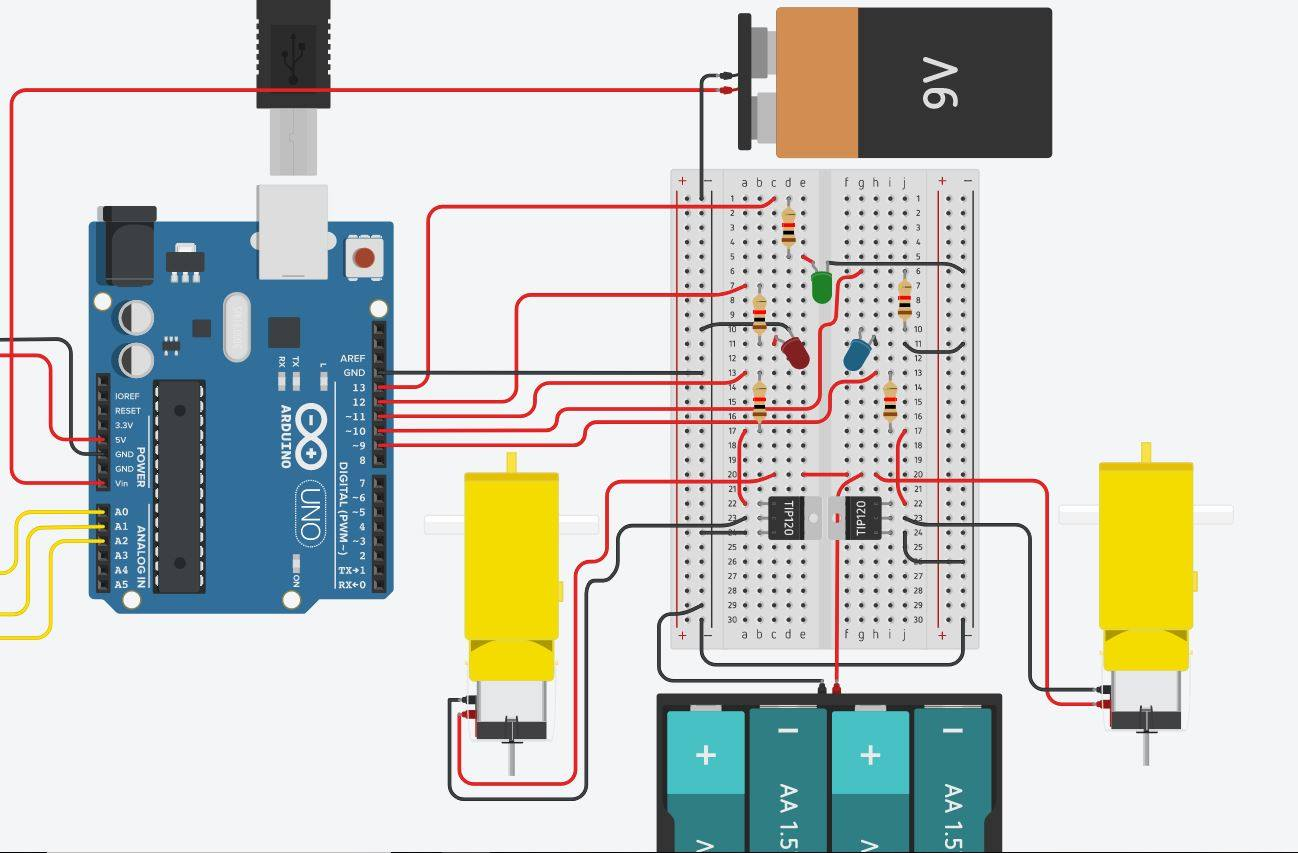
\includegraphics[width=1\columnwidth, keepaspectratio]{CircuitMotors.jpg}
				\caption{Motor and LED Circuit}
				\label{fig:circuitMotors}
			\end{subfigure}
			
			\caption{Circuit schematics for our path following car. In Figure \ref{fig:circuitSensors}, the $1k$ resistors attached to the IR LEDs between the $V_{in}$ and anode ($+$) as well as $10k$ resistors attached to the photo transistors between the emitter and ground. The phototransistors go to Analog pins since their data is transmitted as an analog signal ranging from $0-1000 (arb.)$. In Figure \ref{fig:circuitMotors}, the LEDs are wired the same way as the IR LEDs from before. The TIP120 is connected to $V_{in}$ through a $1k$ resistor on its base, to the motor through its collector, and to ground through its emitter. All of the circuits were created using Tinkercad\cite{tinkercad}.}
			}
		\end{figure}
		
		\vspace{5em}
		
		\hspace{1em}The car goes straight whenever the front sensor triggers low. As soon as either the left or right sensors trigger low, the car turns in the opposite direction (left if right triggers, right if left triggers) until the front sensor again triggers low. The rate at which the car turns back towards the front sensor was adjusted using PID methods\cite{beauregard2011} to allow the car to orient itself along the line both faster and more precisely. After the front sensor triggers low, the car then continues straight again and repeats this process until the stop conditions are met.\\ \hspace{1em}A pulse width modulation (PWM) and transistor are used in conjunction to control the speed of the motor. See Figure \ref{fig:circuitMotors} for the proper wiring. The PWM signal is connected to the base of the transistor and the duty cycle of the PWM is used to control the speed of the motor. Increasing the duty cycle of the PWM increases the speed of the motor by increasing the relative time it is on to that for which it is off. LEDs are used to signal which direction the car is going: a green LED signals forward, a red LED signals left, and a blue LED signals right. In the case of the car’s stopping conditions being met, the car stops moving and then both the blue and red LEDs turn on. LEDs have two sides: a negative (‘n’) side and a positive (‘p’) side. The n side is filled with electrons and the p side is filled with holes. Energy is released when electrons annihilate the holes, with this energy cultivating itself in the form of light. \\ \vspace{1em}
				
						
		\sectionTitle{Testing Methodology}
		
		\subsectionTitle{How We Designed the Test}
		
		\hspace{1em}To obtain a comprehensive test of our path sensing subsystem and sensors, we took a multi step approach by testing the initial, adjusted, and mapped readings from our \textit{getDistance()} function before testing the entire function. Each of our tests involved a setup where the car was propped onto a cardboard jack (e.g. paper roll) and the sensors suspended over a stationary piece of paper that was unmarked besides lines acting as a metric ruler. Using another similarly delineated paper with a  
				
		\begin{figure}[H]
			
			\centering{\textbf{Sensor Testing Rig and Setup}\par\medskip}
			{\begin{subfigure}[t]{0.45\textwidth}
					\frame{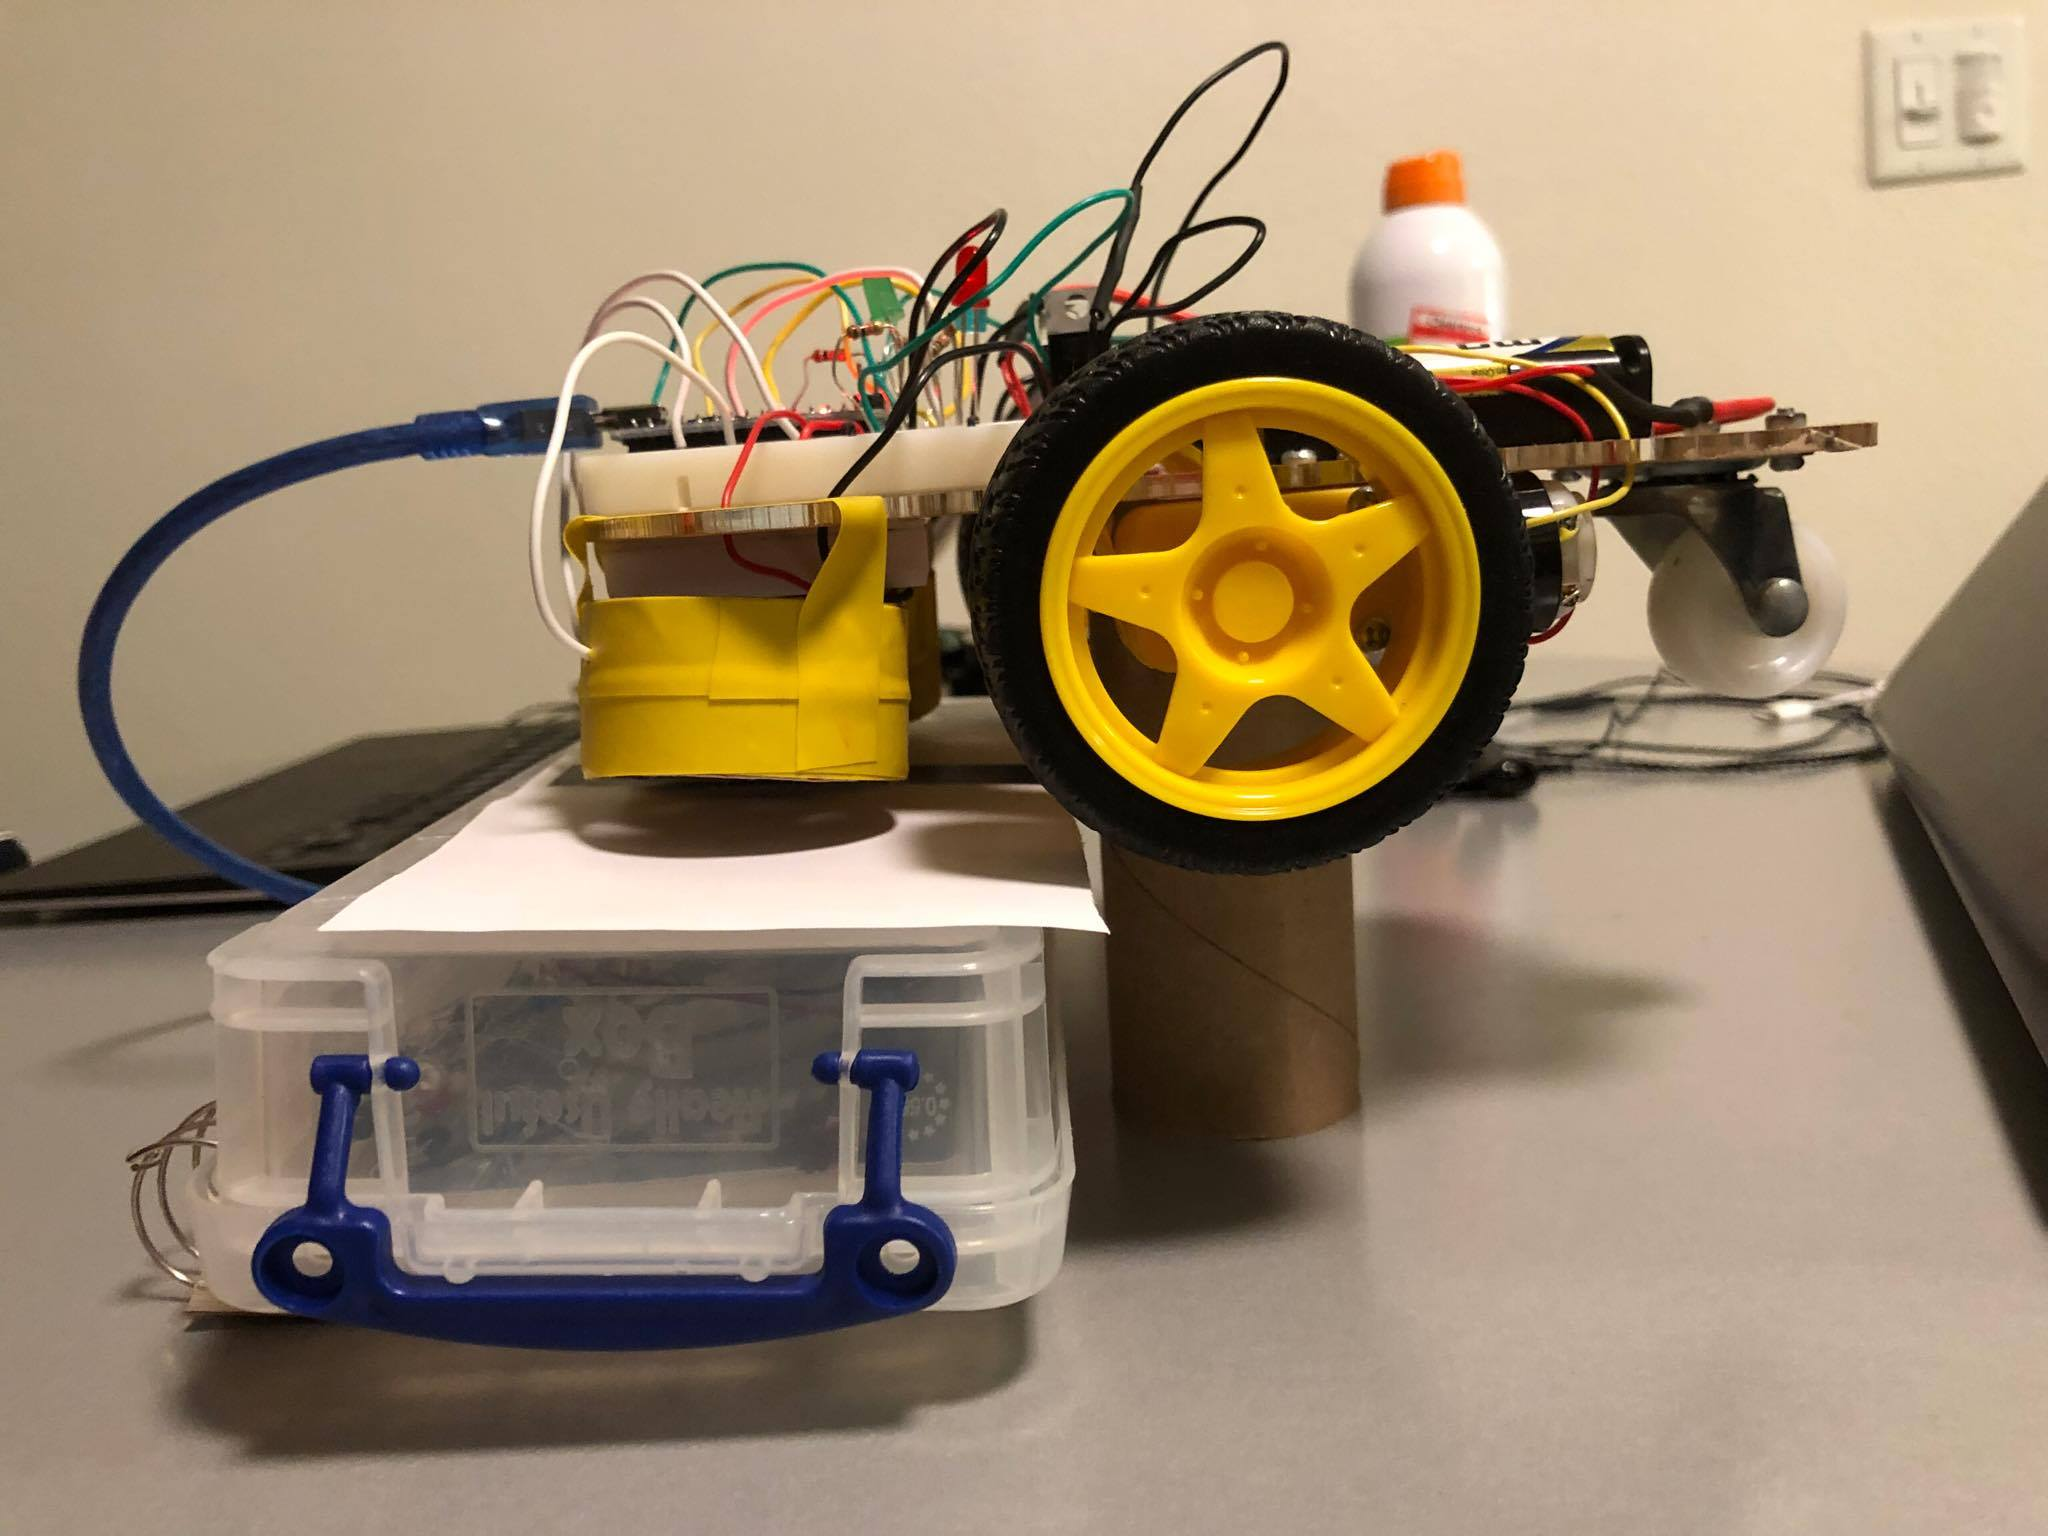
\includegraphics[width=1\columnwidth, keepaspectratio]{TestProcedure_Rig.jpg}}
					\caption{Cardboard Jack}
					\label{fig:procedureRig}
				\end{subfigure}\\ \vspace{1em}%
				\begin{subfigure}[b]{0.45\textwidth}
					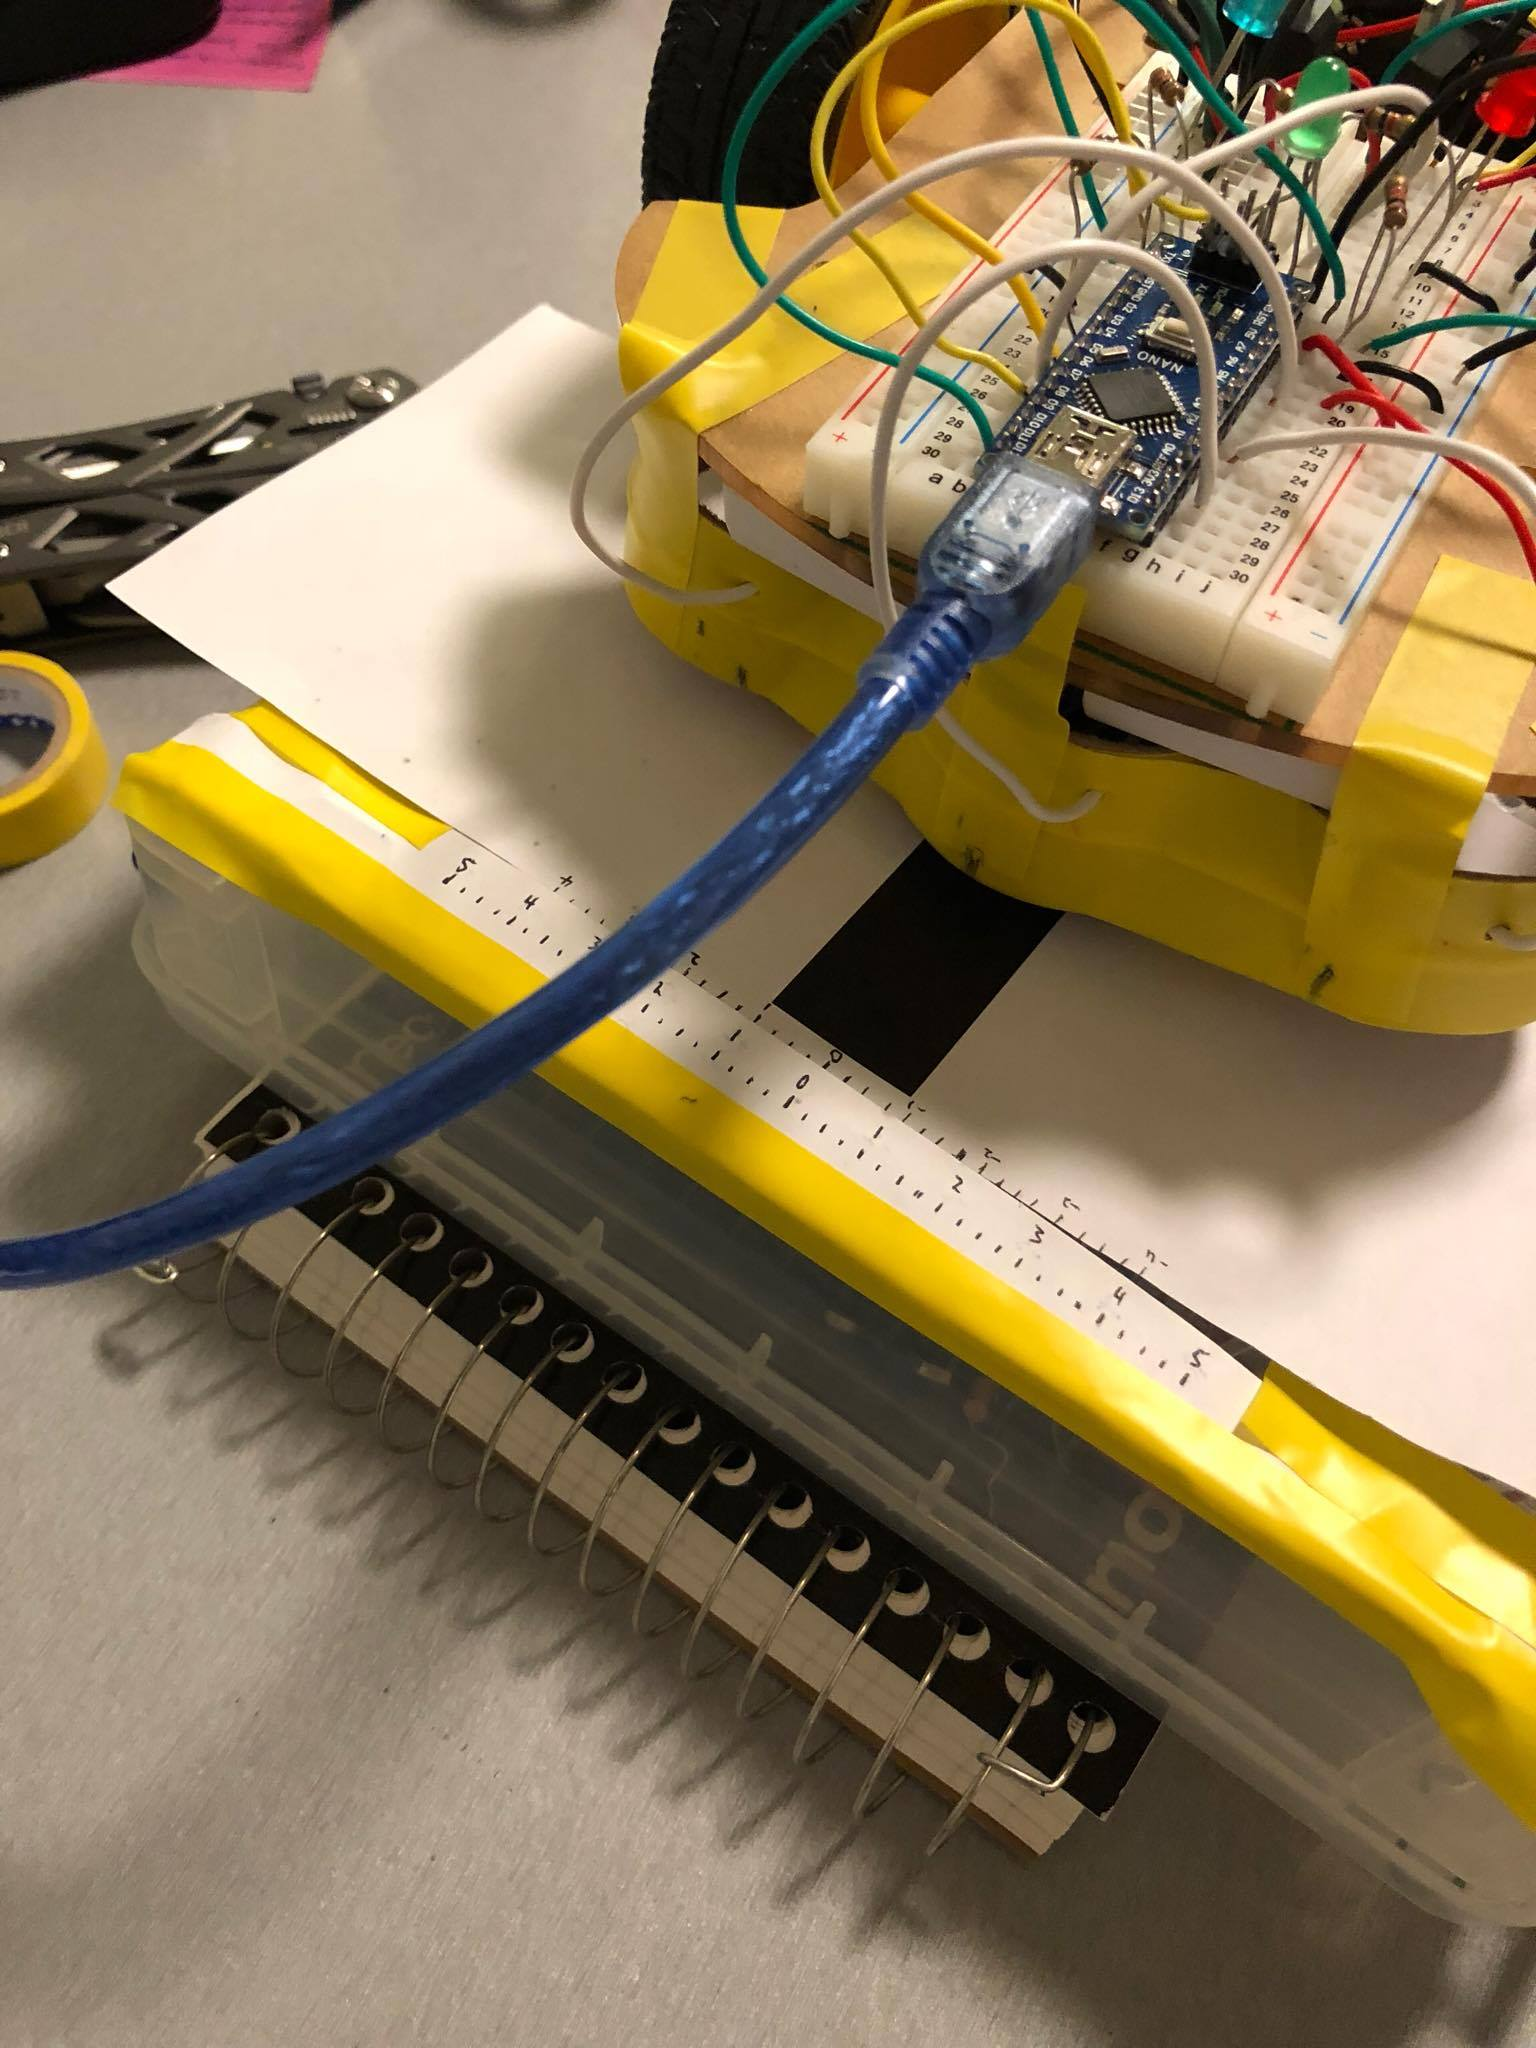
\includegraphics[width=1\columnwidth, keepaspectratio]{TestProcedure_Ruler.jpg}
					\caption{Sliding and Stationary Ruler}
					\label{fig:procedureRuler}
				\end{subfigure}
				
				\caption{Figure \ref{fig:procedureRig} shows how the car was suspended above the ruler. Figure \ref{fig:procedureRuler} shows both rulers; the stationary ruler with a range of \rpm$5cm$ and the sliding ruler with a range of \rpm$4cm$.}
			}
		\end{figure}

		\textit{2cm}-wide black line approximating that of the course’s, we aimed to simulate the car’s motion by moving the line to different distances along the sensor axis. With our setup in place, we began recording values from trials at each of the steps. \\ \vspace{1em}
		
		\subsectionTitle{How We Conducted the Test}

		\hspace{1em}The test was conducted in four parts. For the first three parts, which consisted of the function component tests, we took measurements for each of the sensors separately, centering them on the black line, and measured \rpm\textit{1cm} from the edge of the line. Originally, we measured \rpm\textit{2cm} but noticed that past a centimeter made no difference as the IR phototransistor was unable to read that far away. From these three trials, we were able to tune our processing of the sensor readings to better gauge the distance. Then for the final trial, where we tested the overall \textit{getDistance()} function, we took measurements by going to the right and left sensors (\rpm\textit{4cm}) and taking measurements of the estimated distance at 0.25cm intervals going back to the center. \\ \vspace{1em}
		
		\subsectionTitle{How We Analyzed the Test Data}

		\hspace{1em}After each of our trials, we graphed the estimated distance (function’s output printed to Serial) versus the actual distance (as measured). The first trial gave us a polynomial-looking graph so we found the polynomial regression and solved in terms of \textit{y} in order to obtain a distance value from the sensor reading. Taking new measurements using our newly found formulas gave us the second trial, where after graphing, we noticed our global minima were preserved for each of the sensors but the range condensed. We knew the range was limited as from Trial 1 we found that the sensors could read \rpm\textit{1cm} away. Having adjusted our code once more before our final trial, we moved onto the fourth and final trial, where we graphed all of the sensors on the same axis with \textit{x=0} being the center of the front sensor. From here we began our interpretation of the results. \\ \vspace{3em}
		
		\subsectionTitle{How We Interpreted the Data}

		\hspace{1em}Looking at the trial of the overall performance of the \textit{getDistance()} function, performance was interpreted according to two metrics: absolute error at different points and overall trend. For the sensor function to be acceptable, the distance as output by the function should decrease as the black line goes from the left or right sensor towards the front sensor and reach a minimum once at the direct center of the front sensor and car. In addition to this, we judged success on the difference between the estimated distance and the actual distance. As the sensor can only read a maximum of \textit{1cm} away, we aimed for a maximum error of half that or \textit{0.5cm}. \\ \vspace{1em}

		\sectionTitle{Results and Discussion}
			
		\subsectionTitle{Test Discussion}

		\hspace{1em}Looking at the results of our first trial as seen in Figure \ref{graph:sRaw}, we were able to fit a polynomial regression to the readings from each sensor fairly well, with a minimum $r^2$ value of $0.927$ and a maximum $r^2$ value of $0.989$. From there, our first attempt at obtaining the distance from line based on sensor readings was too compressed in range but after mapping looked to approximate each sensor relatively well. This was confirmed by our second and third trials in Figure \ref{graph:sMapped} where by using the polynomial fit we had the correct magnitude but only after mapping did we have the correct range. However, once we ran our final trial and looked at the data our function was clearly lacking in `blind zones' between the front and side sensors (\textit{-1.25cm} to \textit{-2.75cm} on the left and \textit{1cm} to \textit{3cm} on the right). This was to be expected, however, as using only three sensors across such a large range limits the line of sight. Regardless of this, the function performed well for the other values which were within range of a sensor and gave us a maximum error of about \textit{0.5cm}. See the section entitled \textbf{`Tables and Graphs'} for the figures referenced in this previous section.\\ \vspace{4em}
		
		\subsectionTitle{Race Day Results}

		\hspace{1em}On our test day, our car completed the \textit{~20ft} course containing four \textit{90 degree} turns and five straight sections in \textit{29.7 seconds}. Originally it completed the course in \textit{33.4 seconds} but with some adjustments we were able to get it going faster on this specific track by adjusting our PID constants and base speed. \\ \vspace{1em}
			
		\sectionTitle{Conclusions and Future Work}
			
		\hspace{1em}Our project met the objective of following path fairly well. Despite the fact that it did so in a non-ideal manner by moving along the path sinusoidally, the car never deviated too far away from the path. In addition, we were also able to complete an additional goal of the project which was to detect a stopped wheel by using a photomicrosensor. One thing we learned during the project is the value of being able to read datasheets and using them to create an organized circuit. Keeping the circuit organised not only helps whenever we are trying to figure out wiring issues, but also keeps live wires from touching each other and potentially shorting or otherwise damaging a circuit component. Another thing we learned was how to effectively use a PID function to help with differential steering, and the procedure to test and find the constants for our PID method. Based on how quickly and accurately the car is able to track the center line, we know whether or not the PID constants $k_p$, $k_d$, or $k_i$ need to be adjusted. \\ \vspace{1em}
		
		\hspace{1em}Given more time, an extension we would like to have done is test different configurations of sensors instead of being limited to using three. By testing other sensor layouts we could have potentially solved the issue of having a `blind zone’ that we found during our sensor subsystem tests. This would increase the accuracy of which our car can measure distance as there optimally wouldn’t be an area for which no sensor can obtain a reading. Our PID function would see an improvement from this and could also be better tuned since error calculation would be more responsive and precise. We would test this improvement by using the same method we tested our three sensor subsystem as it not only allows us to see the accuracy but also tune the function in the process. \\ \vspace{-54em}

		\setlength\bibitemsep{0pt}
		\printbibliography[title={\uline{\large{References}}\vspace{-14em}}] 

		\pagebreak
		\sectionTitle{Tables and Graphs}
		
		\vspace{0em}
	
		\begin{table}[H]
			\centering{\textbf{Raw Data from Sensors}\par\medskip}
			\pgfplotstabletypeset[
			column type=,
			begin table={\begin{tabularx}{.8\columnwidth}{D{.}{.}{0} X X X}},
				end table={\end{tabularx}},
			col sep=comma,
			columns/d/.style={{column name=\textbf{Distance} $\ (cm.)$}, fixed, fixed zerofill, precision=2},
			columns/l/.style={column name=Left},
			columns/f/.style={column name=Front},
			columns/r/.style={column name=Right},
			every head row/.style={before row={
					\toprule
					\multicolumn{1}{c}{} & \multicolumn{3}{c}{\textbf{Sensor Values} $(arb.)$}\\
					\cmidrule{2-4}
				},after row=\toprule},
			every last row/.style={after row=\bottomrule},
			]{sensorsRaw.csv}
			\caption{Readings obtained from each of the sensors during Trial 1 by printing to \textit{Serial.Out()}.
				\vspace{13em}}
		\end{table}

		\begin{table*}[p]
			\ra{1.3}
			\centering{\textbf{Adjusted and Mapped Distance from Sensors}\par\medskip}
			\pgfplotstabletypeset[
			column type=,
			begin table={\begin{tabularx}{1.5\columnwidth}{D{.}{.}{0} X X X X X X}},
				end table={\end{tabularx}},
			col sep=comma,
			columns/d/.style={{column name={\textbf{Distance} $\ (cm.)$}}, fixed, fixed zerofill, precision=2},
			columns/lr/.style={column name=Left}, fixed, fixed zerofill, precision=2,	columns/fr/.style={column name=Front}, fixed, fixed zerofill, precision=2,
			columns/rr/.style={column name=Right}, fixed, fixed zerofill, precision=2,
			columns/lm/.style={column name=Left}, fixed, fixed zerofill, precision=2,
			columns/fm/.style={column name=Front}, fixed, fixed zerofill, precision=2,
			columns/rm/.style={column name=Right}, fixed, fixed zerofill, precision=2,
			every head row/.style={before row={
					\toprule
					\multicolumn{1}{c}{} & \multicolumn{3}{c}{\textbf{Distance, Adjusted $(cm.)$}} & \multicolumn{3}{c}{\textbf{Distance, Mapped $(cm.)$}}\\
					\cmidrule(lr){2-4} \cmidrule(lr){5-7}
				},after row=\toprule},
			every last row/.style={after row=\bottomrule},
			]{sensorsMapped.csv}
			\caption{Readings obtained from Trial 2 and Trial 3 where each sensor was tested individually.}
		\end{table*}

		\begin{table*}[p]
			\ra{1.1}
			\centering{\textbf{Final Trial of Distance Function}\par\medskip}
			\pgfplotstabletypeset[
			column type=,
			begin table={\begin{tabularx}{1.2\columnwidth}{D{.}{.}{0} c c}},
				end table={\end{tabularx}},
			col sep=comma,
			columns/d/.style={{column name={\textbf{Distance} $\ (cm.)$}}, fixed, fixed zerofill, precision=2},
			columns/a/.style={column name={\textbf{Actual} $\ (cm.)$}}, fixed, fixed zerofill, precision=2,
			columns/m/.style={column name={\textbf{Measured} $\ (cm.)$}}, fixed, fixed zerofill, precision=2,
			every head row/.style={before row=\toprule, after row=\toprule},
			every last row/.style={after row=\bottomrule},
			]{sensorsTest.csv}
			\caption{Readings from our test of the overall sensor-based line detecting system in the fourth and final Trial.}
		\end{table*}

		\begin{figure*}[p]
			\centering{
				\centering{\textbf{Raw Data From Sensors}\par\medskip}
				\begin{subfigure}{\columnwidth}
					\centering
					\begin{tikzpicture}[
					every node/.style={text=black},
					fdesc/.default=1
					]
					
					\pgfplotsset{
						width=2.5in,
						height=2.5in,
						legend style={cells={align=left}, at={(axis cs:1.8,50)},anchor=south east, font=\footnotesize}
					}
					\begin{axis}[
					xlabel={Distance from Line, $cm$ ($centimeters$).},
					ylabel={Sensor Reading, $value$ ($arb.$).},
					xmin=-2, xmax=2,
					xtick distance=1,
					ymin=0, ymax=1000,
					ytick distance=200,
					]
					
					%% Marks %%
					\addplot [
					color=black,
					mark=*,
					mark options={fill=black},
					mark size=1pt,
					forget plot
					] table [col sep=comma, y=f, x=d]{sensorsRaw.csv};
					
					%% Polynomic Regression
					\addplot [color=red, smooth] {652*x*x+166*x+499};
					\addlegendentry{$652x^2+166x+499$\\$r^2=0.989$};
					
					\end{axis}
					\end{tikzpicture}
					\caption{Front Sensor}
					\vspace{0.5em}
					\label{graph:sRawFront}
				\end{subfigure}\\
				\begin{subfigure}{\columnwidth}
					\centering
					\begin{tikzpicture}[
					every node/.style={text=black},
					fdesc/.default=1
					]
					
					\pgfplotsset{
						width=2.5in,
						height=2.5in,
						legend style={cells={align=left}, at={(axis cs:1.8,50)},anchor=south east, font=\footnotesize}
					}
					\begin{axis}[
					xlabel={Distance from Line, $cm$ ($centimeters$).},
					ylabel={Sensor Reading, $value$ ($arb.$).},
					xmin=-2, xmax=2,
					xtick distance=1,
					ymin=0, ymax=1000,
					ytick distance=200,
					]
					
					\addplot [
					color=black,
					mark=*,
					mark options={fill=black},
					mark size=1pt,
					forget plot
					] table [col sep=comma, y=l, x=d]{sensorsRaw.csv};
					
					%% Polynomic Regression
					\addplot [color=red, smooth] {355*x*x+32*x+625};
					\addlegendentry{$355x^2+32x+625$\\$r^2=0.951$};
					
					\end{axis}
					\end{tikzpicture}
					\caption{Left Sensor}
					\label{graph:sRawLeft}
				\end{subfigure}\hfill
				\begin{subfigure}{\columnwidth}
					\centering
					\begin{tikzpicture}[
					every node/.style={text=black},
					fdesc/.default=1
					]
					
					\pgfplotsset{
						width=2.5in,
						height=2.5in,
						legend style={cells={align=left}, at={(axis cs:1.8,50)},anchor=south east, font=\footnotesize}
					}
					\begin{axis}[
					xlabel={Distance from Line, $cm$ ($centimeters$).},
					ylabel={Sensor Reading, $value$ ($arb.$).},
					xmin=-2, xmax=2,
					xtick distance=1,
					ymin=0, ymax=1000,
					ytick distance=200,
					]
					
					%% Marks %%
					\addplot [
					color=black,
					mark=*,
					mark options={fill=black},
					mark size=1pt,
					forget plot
					] table [col sep=comma, y=r, x=d]{sensorsRaw.csv};
					
					%% Polynomic Regression
					\addplot [color=red, smooth] {626*x*x-23*x+301};
					\addlegendentry{$626x^2-23x+301$\\$r^2=0.927$};
					
					\end{axis}
					\end{tikzpicture}
					\caption{Right Sensor}
					\label{graph:sRawRight}
				\end{subfigure}
				\caption{\textbf{Raw readings from the IR sensor, IR phototransistor combinations used on our path-following robot.} From the graphs, the value of the maximum readings range from about $400$ for Graph \ref{graph:sMappedRight} to about $600$ for Graph \ref{graph:sMappedLeft}. Also worth noting is that the sensors each reach trend down to a global minimum of around $0cm$ when moving from \rpm$1cm$ to the black line.}\label{graph:sRaw}
			}
		\end{figure*}
		
		\begin{figure*}[p]
			\centering{
				
				\centering{\textbf{Adjusted and Mapped Distances From Sensors}\par\medskip}
				
				\begin{subfigure}{\columnwidth}
					\centering
					\begin{tikzpicture}[
					every node/.style={text=black},
					fdesc/.default=1
					]
					
					\pgfplotsset{
						width=2.5in,
						height=2.5in,
						legend style={font=\footnotesize}
					}
					\begin{axis}[
					xlabel={Distance from Line, $cm$ ($centimeters$).},
					ylabel={Adjusted Sensor Reading, $value$ ($arb.$).},
					xmin=-1, xmax=1,
					xtick distance=0.5,
					ymin=0, ymax=1,
					ytick distance=0.2,
					]
					
					%% Marks %%
					\addplot [
					color=black,
					mark=*,
					mark options={fill=black},
					mark size=1pt
					] table [col sep=comma, y=fr, x=d]{sensorsMapped.csv};
					
					\addplot [
					color=blue,
					mark=*,
					mark options={fill=blue},
					mark size=1pt
					] table [col sep=comma, y=fm, x=d]{sensorsMapped.csv};
					
					\end{axis}
					\end{tikzpicture}
					\caption{Front Sensor}
					\vspace{0.5em}
					\label{graph:sMappedFront}
				\end{subfigure}\\%
				\begin{subfigure}{\columnwidth}
					\centering
					\begin{tikzpicture}[
					every node/.style={text=black},
					fdesc/.default=1
					]
					
					\pgfplotsset{
						width=2.5in,
						height=2.5in,
						legend style={font=\footnotesize}
					}
					\begin{axis}[
					xlabel={Distance from Line, $cm$ ($centimeters$).},
					ylabel={Adjusted Sensor Reading, $value$ ($arb.$).},
					xmin=-1, xmax=1,
					xtick distance=0.5,
					ymin=0, ymax=1,
					ytick distance=0.2,
					]
					
					\addplot [
					color=black,
					mark=*,
					mark options={fill=black},
					mark size=1pt
					] table [col sep=comma, y=lr, x=d]{sensorsMapped.csv};
					
					%% Marks %%
					\addplot [
					color=blue,
					mark=*,
					mark options={fill=blue},
					mark size=1pt
					] table [col sep=comma, y=lm, x=d]{sensorsMapped.csv};
					
					\end{axis}
					\end{tikzpicture}
					\caption{Left Sensor}
					\label{graph:sMappedLeft}
				\end{subfigure}%
				\hfill
				\begin{subfigure}{\columnwidth}
					\centering
					\begin{tikzpicture}[
					every node/.style={text=black},
					fdesc/.default=1
					]
					
					\pgfplotsset{
						width=2.5in,
						height=2.5in,
						legend style={font=\footnotesize}
					}
					\begin{axis}[
					xlabel={Distance from Line, $cm$ ($centimeters$).},
					ylabel={Adjusted Sensor Reading, $value$ ($arb.$).},
					xmin=-1, xmax=1,
					xtick distance=0.5,
					ymin=0, ymax=1,
					ytick distance=0.2,
					]
					
					%% Marks %%
					\addplot [
					color=black,
					mark=*,
					mark options={fill=black},
					mark size=1pt
					] table [col sep=comma, y=rr, x=d]{sensorsMapped.csv};
					
					%% Marks %%
					\addplot [
					color=blue,
					mark=*,
					mark options={fill=blue},
					mark size=1pt
					] table [col sep=comma, y=rm, x=d]{sensorsMapped.csv};
					\end{axis}
					\end{tikzpicture}
					\caption{Right Sensor}
					\label{graph:sMappedRight}
				\end{subfigure}
				\caption{\textbf{Adjusted sensor readings using a crude polynomial fit of the data from Graphs \ref{graph:sRawFront}, \ref{graph:sRawLeft}, and \ref{graph:sRawRight} with a degree $n=2$ and then mapping to expand the range across the sensors line of sight ($0$ to $1cm$).} By using a polynomial fit of the sensor reading ($y$) versus the distance from the line ($x$) and solving in terms $y$, we are able to both find the distance from our readings and preserve each sensors local minimum at $0cm$. From there, we need to adjust the values to fit our known distribution and therefore simply map it as shown. By doing this, we see that our data better fits the distribution and is able to give us more valuable information to use with our PID function as the same change in the sensor reading returns a more significant change (and accurate) change in calculated distance from the line.}\label{graph:sMapped}
			}
		\end{figure*}
		
		\begin{figure*}[p]
			\centering{
				
				\centering{\textbf{Final Trial of Distance Function}\par\medskip}
				
				\begin{tikzpicture}[
				every node/.style={text=black},
				fdesc/.default=1
				]
				
				\pgfplotsset{
					width=5in,
					height=5in,
					legend style={font=\footnotesize}
				}
				\begin{axis}[
				xlabel={Distance From Line, $cm$ ($centimeters$).},
				ylabel={Absolute Distance From Line, $cm$ ($centimeters$).},
				%			xmin=-1.25, xmax=1.25,
				%			xtick distance=0.5,
				%			ymin=-0.08, ymax=0.07,
				%			ytick distance=0.03,
				xticklabel style={
					/pgf/number format/fixed,
					/pgf/number format/precision=2
				},
				scaled x ticks=false,
				yticklabel style={
					/pgf/number format/fixed,
					/pgf/number format/precision=2
				},
				scaled y ticks=false,
				]
				
				%% Marks %%
				\addplot [
				color=blue,
				mark=*,
				mark options={fill=blue},
				mark size=0.5pt,
				] table [col sep=comma, y=m, x=d]{sensorsTest.csv};
				\addlegendentry{Actual Distance};
				
				\addplot [
				color=black,
				mark=*,
				mark options={fill=black},
				mark size=0.5pt,
				] table [col sep=comma, y=a, x=d]{sensorsTest.csv};
				\addlegendentry{Calculated Distance};
				
				\draw [name path=leftBoundLeft, dashed, red] (-2.75,0) -- (-2.75,4);
				\draw [name path=leftBoundRight, dashed, red] (-1.25,0) -- (-1.25,4);
				\addplot [red!70!white,fill opacity=.2] fill between[
				of=leftBoundLeft and leftBoundRight];
				
				\draw [name path=rightBoundLeft, dashed] (3,0) -- (3,4);
				\draw [name path=rightBoundRight, dashed, red] (1,0) -- (1,4);
				\addplot [red!70!white,fill opacity=.2] fill between[
				of=rightBoundLeft and rightBoundRight] ;
				
				\end{axis}
				\end{tikzpicture}
				\caption{Comparison between actual and measured distance (from our getLocation() function) between center of $2cm$ thin black line and center of robot's front sensor. The red zone in the figure represent the area for which the black line is not within the range of the left, front, or right sensors. The calculated distance for these areas is just the average value of the actual distance. Looking at this graph, the calculated distance is generally accurate to within less than half a centimeter. Most importantly, the graph slopes to a minimum from both sides, an important feature if a function is to be used for a PID controller.}\label{graph:sensorTest}
				\vspace{0.5em}
			}
		\end{figure*}

	\end{flushleft}
	
\end{document}